\documentclass[pdf]{prosper}
\usepackage[Lakar]{HA-prosper}
\usepackage{graphicx}


\begin{document}

\begin{slide}{Principal components and factor analysis}

  \begin{itemize}
  \item Principal components: 
    \begin{itemize}
    \item Purely mathematical.
    \item Find eigenvalues, eigenvectors of correlation matrix.
    \item No testing whether observed components reproducible, or even probability model behind it.
    \end{itemize}
  \item Factor analysis: 
    \begin{itemize}
    \item some way towards fixing this (confirmatory factor analysis, later, a long way).
    \item In factor analysis, each variable modelled as: ``common factor'' (eg. verbal ability) and ``specific factor'' (left over).
    \item SAS: choose the common factors to ``best'' reproduce pattern seen in correlation matrix.
    \item Iterative procedure, different answer from principal components.
    \end{itemize}

  \end{itemize}

\end{slide}

\begin{slide}{Example}

  \begin{itemize}
  \item 
145 children given 5 tests, called PARA, SENT, WORD, ADD and DOTS. 3 linguistic tasks (paragraph comprehension, sentence completion  and word meaning), 2 mathematical ones (addition and counting dots).
\item Correlation matrix:

\begin{verbatim}
para 1     0.722 0.714 0.203 0.095
sent 0.722 1     0.685 0.246 0.181
word 0.714 0.685 1     0.170 0.113
add  0.203 0.246 0.170 1     0.585
dots 0.095 0.181 0.113 0.585 1
\end{verbatim}

\item Is there small number of underlying ``constructs'' (unobservable) that explains this pattern of correlations?
\item First item on each line is name of variable: use SAS special variable \verb-_name_- to read these in.
\item First task: figure out number of factors:
  \begin{itemize}
  \item again can count eigenvalues $>1$
  \item draw {\em scree plot} and look for ``elbow''.
  \end{itemize}


  \end{itemize}
  
\end{slide}

\begin{slide}{Code}

\begin{verbatim}
data rmat(type=corr);
  infile "rex2.dat";
  input _name_ $ para sent word add dots;

proc factor scree method=prinit;

\end{verbatim}

  \begin{itemize}
  \item Names on INPUT line same as names of variables in file.
  \item On PROC FACTOR line, specify method of extracting factors (there are others) and ask for scree plot.
  \item As in principal components, can ask for output data set containing factor scores, but:
    \begin{itemize}
    \item only if have actual data rather than correlations
    \item only goal for this run of PROC FACTOR is to determine a good number of factors.
    \end{itemize}
  \end{itemize}
  
\end{slide}

\begin{slide}{Output}

Start with eigenvalues:

{\scriptsize
\begin{verbatim}
            Preliminary Eigenvalues: Total = 5  Average = 1
 
             Eigenvalue    Difference    Proportion    Cumulative

        1    2.58746987    1.16575215        0.5175        0.5175
        2    1.42171772    1.00652661        0.2843        0.8018
        3    0.41519110    0.10409071        0.0830        0.8849
        4    0.31110040    0.04657948        0.0622        0.9471
        5    0.26452092                      0.0529        1.0000

        2 factors will be retained by the MINEIGEN criterion.
\end{verbatim}
}

2 eigenvalues bigger than 1, so SAS keeps 2 factors. 80\% of variability explained by these, not bad.

  
\end{slide}

\begin{slide}{Scree plot}
  
{\tiny
\begin{verbatim}
Scree Plot of Eigenvalues
  3 +
    |
E   |                 1
i   |
g   |
e 2 +
n   |
v   |
a   |                           2
l   |
u 1 +
e   |
s   |
    |                                     3         4
    |                                                         5
  0 +
    |
    --------+---------+---------+---------+---------+---------+-------
            0         1         2         3         4         5

                                  Number
\end{verbatim}
}

Looking for where plot ``turns corner'' or ``has elbow'': at 3rd eigenvalue, so keep $3-1=2$ factors.

\end{slide}

\begin{slide}{Eigenvalues of reduced correlation matrix}

After SAS has finished iterating, the eigenvalues are different:

{\scriptsize
\begin{verbatim}
            Eigenvalues of the Reduced Correlation Matrix:
               Total = 3.31477718  Average = 0.66295544
 
             Eigenvalue    Difference    Proportion    Cumulative

        1    2.28220070    1.25031114        0.6885        0.6885
        2    1.03188956    1.00687378        0.3113        0.9998
        3    0.02501578    0.02604204        0.0075        1.0073
        4    -.00102626    0.02227632       -0.0003        1.0070
        5    -.02330258                     -0.0070        1.0000

\end{verbatim}
}

Sometimes they are slightly negative, but this is nothing to worry about. 

\vspace{2ex}

SAS chose 2 factors, so other eigenvalues very close to 0.

  
\end{slide}

\begin{slide}{Factor pattern and communality estimates}

{\scriptsize
\begin{verbatim}
                           Factor Pattern
 
                              Factor1         Factor2
                 para         0.83498        -0.24200
                 sent         0.82533        -0.13946
                 word         0.78992        -0.22671
                 add          0.40982         0.63174
                 dots         0.33454         0.70949
\end{verbatim}
}

Factor 1 mostly ``words'' and factor 2 mostly ``numbers'', but could be clearer. Called ``factor loadings'', easier to interpret if close to 0 or $\pm 1$.

{\scriptsize
\begin{verbatim}
             Final Communality Estimates: Total = 3.314090
       para           sent           word            add           dots
0.75574929     0.70062380     0.67537332     0.56705315     0.61529069
\end{verbatim}
}

Show how each variable related to the factors (jointly): a low communality means the variable concerned not related to any of the factors. Here, though, all communalities reasonably high. (Actually R-squareds from regression of variable on factor.)
  
\end{slide}

\begin{slide}{What to do next}

  \begin{itemize}
  \item 2 factors appears to be good. No longer worry about scree plot or getting SAS to choose: we specify.
  \item {\em Factor rotation:}
    \begin{itemize}
    \item So far, choose 1st factor to maximize spread, and 2nd factor ditto, while unrelated to 1st factor.
    \item Now know we'll have 2 factors, so choose them to jointly maximize spread.
    \item Introduces extra ``degree of freedom'', can use to get ``interpretable'' factors by idea of {\em factor rotation}.
    \item {\em Varimax} rotation tries to drive {\em columns} of factor pattern close to 0 or $\pm 1$.
    \item {\em Quartimax} rotation tries to arrange that each variable only appears in {\em one} factor.
    \end{itemize}
  \end{itemize}
  
\end{slide}

\begin{slide}{More code}

Replace previous PROC FACTOR call with following:

\begin{verbatim}
proc factor n=2 method=prinit rotate=varimax;
\end{verbatim}

We decide on 2 factors, ask for varimax rotation.

\vspace{3ex}

Produces output from before plus following:
  
\end{slide}

\begin{slide}{Rotated factors}

{\scriptsize
\begin{verbatim}
                        Rotated Factor Pattern
 
                              Factor1         Factor2

                 para         0.86556         0.08098
                 sent         0.81899         0.17284
                 word         0.81804         0.07868
                 add          0.14966         0.73801
                 dots         0.05112         0.78274
\end{verbatim}
}

Now rather clearer that factor 1 is verbal ability and factor 2 mathematical.

{\scriptsize
\begin{verbatim}
             Final Communality Estimates: Total = 3.314090
 
      para           sent           word            add           dots
0.75574929     0.70062380     0.67537332     0.56705315     0.61529069
\end{verbatim}
}

Communalities unaffected by rotation.
  
\end{slide}

\begin{slide}{A bigger example: BEM sex role inventory}

  \begin{itemize}
  \item 369 women asked to rate themselves on 44 traits, like ``self-reliant'' or ``shy''.
  \item Rating 1 ``never or almost never true of me'' to 7 ``always or almost always true of me''.
  \item 44 personality traits is a lot. Can we find a smaller number of factors that capture aspects of personality?
  \item The whole BEM sex role inventory on next page.
  \end{itemize}
  
\end{slide}

\begin{slide}{The whole inventory}

{\centering
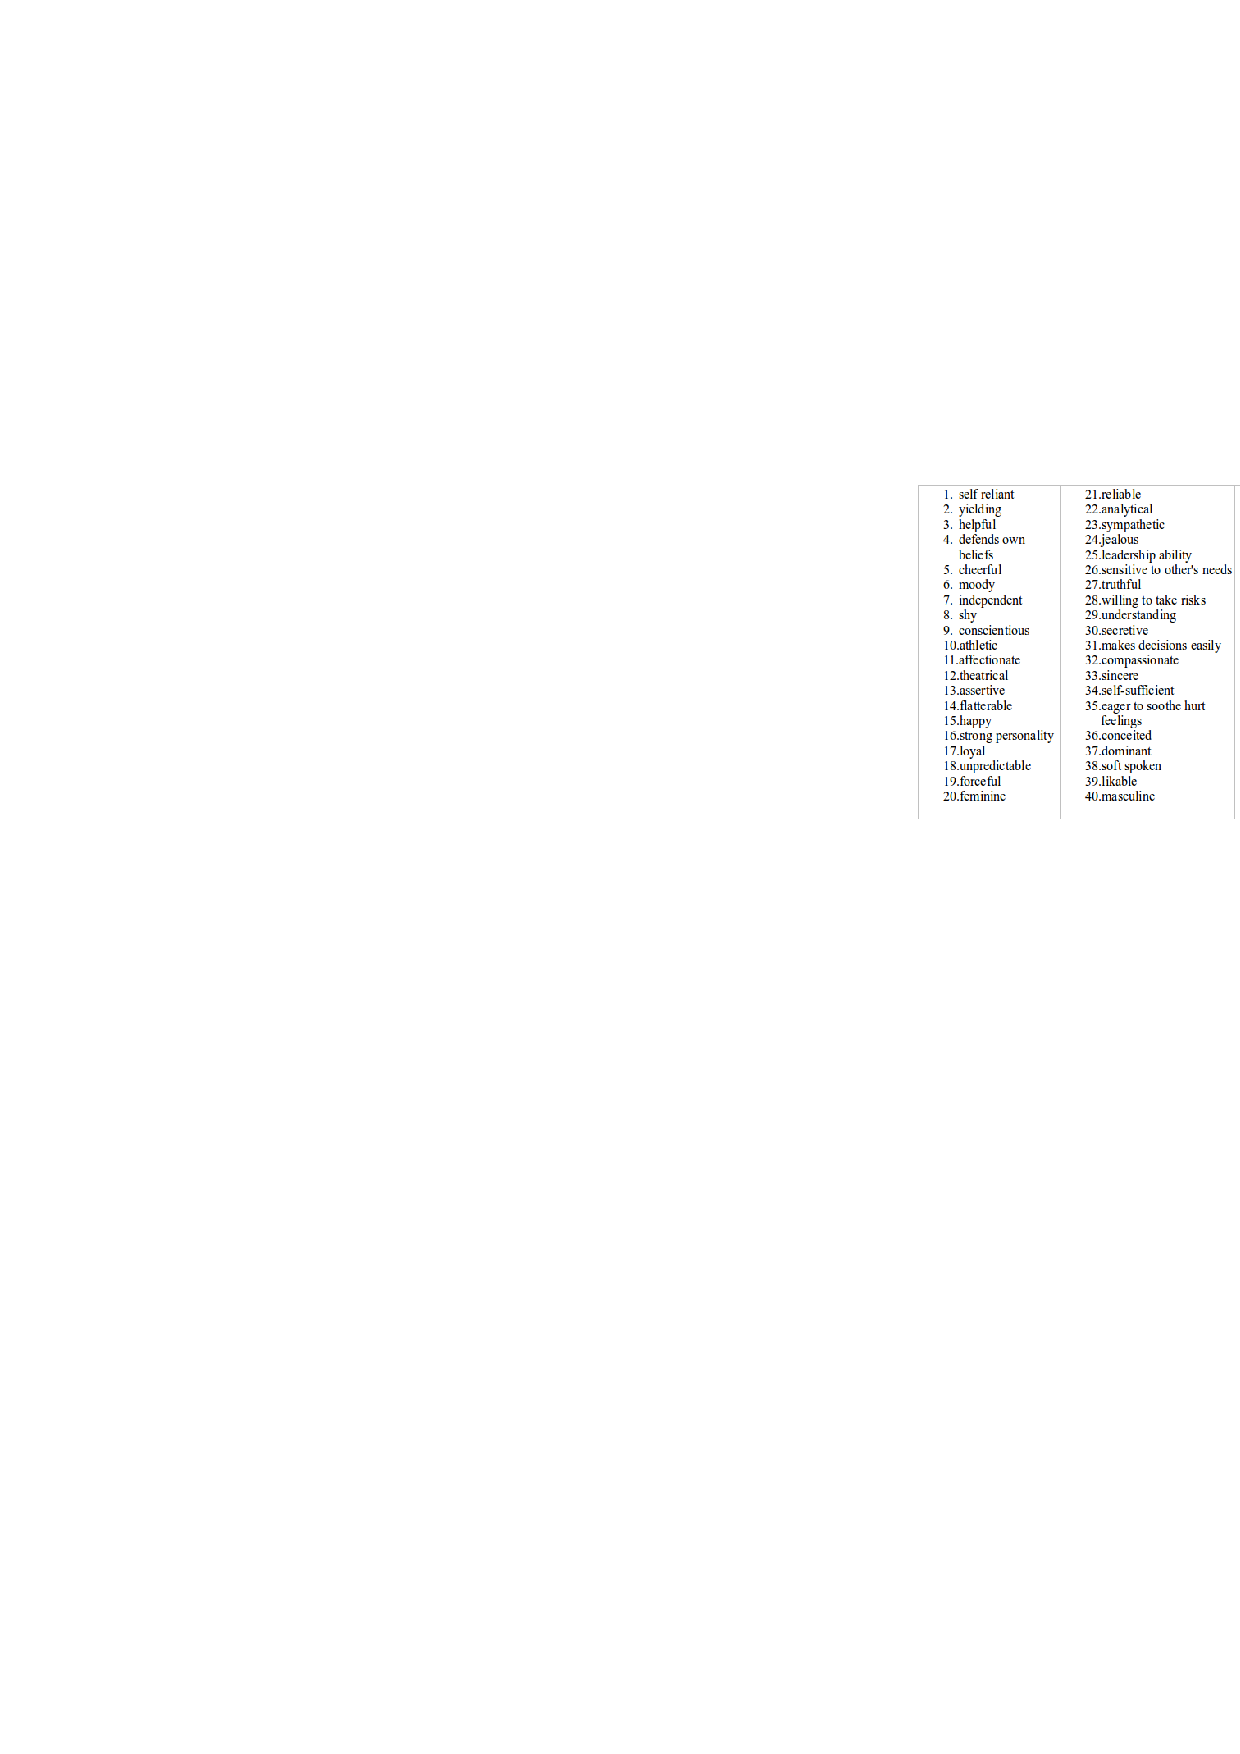
\includegraphics[width=4.5in]{bem}
  }

\end{slide}

\begin{slide}{Reading a SAS data set}

  \begin{itemize}
  \item Data come to us as a SAS data set (somebody else has read the numbers in from a file and created a SAS data set, which they saved).
  \item First step is to specify the \verb-libname-, where the data set file is, which is usually in same folder as code. This can be given any name, like \verb-fred-, resulting in 

\begin{verbatim}
libname fred '.';
\end{verbatim}

  \item Then data step only needs to contain one line (no infile, input etc):

\begin{verbatim}
data x;
  set fred.datasetname;
\end{verbatim}

links our SAS data set \verb-x- to SAS data set file \verb-datasetname- in current directory (folder).
\end{itemize}
\end{slide}

\begin{slide}{More; number of factors}

\begin{itemize}
\item
In our case, data in file \verb-factor.sas7bdat-, so code as below. Also, data step can contain other things like defining new variables. In our case, data file contains variable \verb-subno-, which we don't want:

\begin{verbatim}
libname sasdata '.';

data bem;
  set sasdata.factor;
  drop subno;

\end{verbatim}

  \item Run PROC FACTOR with scree plot, look at eigenvalues.
  \item No rotation yet, since interpretation later. 

\begin{verbatim}
proc factor scree method=prinit;
\end{verbatim}
  \end{itemize}


\end{slide}

\begin{slide}{Scree plot}

{\tiny
\begin{verbatim}
Scree Plot of Eigenvalues
      |
  7.5 +     1
      |
E     |
i     |
g     |
e 5.0 +      2
n     |
v     |
a     |
l     |
u 2.5 +        3
e     |         4
s     |          567
      |              89012 34567 89
      |                            012 34567 89012 34567 89012
  0.0 +                                                        34
      |
      -----+-----+-----+-----+-----+-----+-----+-----+-----+-----+----
           0     5    10    15    20    25    30    35    40    45

                                   Number

\end{verbatim}
}

Scale makes it hard to tell, but might be an elbow at 5, favouring 4 factors.
  
\end{slide}

\begin{slide}{The eigenvalues}

{\scriptsize
\begin{verbatim}
           Preliminary Eigenvalues: Total = 44  Average = 1
 
             Eigenvalue    Difference    Proportion    Cumulative

        1    7.53227628    2.51208242        0.1712        0.1712
        2    5.02019387    2.61617135        0.1141        0.2853
        3    2.40402251    0.33369433        0.0546        0.3399
        4    2.07032818    0.37202817        0.0471        0.3870
        5    1.69830001    0.28605615        0.0386        0.4256
        6    1.41224387    0.06851943        0.0321        0.4577
        7    1.34372444    0.18080134        0.0305        0.4882
        8    1.16292310    0.01544149        0.0264        0.5146
        9    1.14748161    0.04705296        0.0261        0.5407
       10    1.10042865    0.02197431        0.0250        0.5657
       11    1.07845434    0.07540628        0.0245        0.5902
       12    1.00304806    0.04746411        0.0228        0.6130
       13    0.95558395    0.03978141        0.0217        0.6348
       14    0.91580253    0.05321790        0.0208        0.6556
       15    0.86258464    0.01134500        0.0196        0.6752
       16    0.85123963    0.03066264        0.0193        0.6945
       ...
       43    0.23079710    0.08266928        0.0052        0.9966
       44    0.14812782                      0.0034        1.0000
\end{verbatim}
}

\end{slide}
\begin{slide}{Interpreting eigenvalues}

\begin{itemize}
\item 
No ``obvious'' gaps -- maybe first 2 eigenvalues bigger than others (but then only 28.5\% of variability explained).
\item Scree plot said 4 eigenvalues before ``elbow''.
\item 12 eigenvalues $>1$, even then only 61.3\% of variability explained.
\item Personality is complicated, multidimensional thing.
\end{itemize}
  
\end{slide}

\begin{slide}{Extract 4 factors for interpretation}

  \begin{itemize}
  \item Specify to extract 4 factors.
  \item Aim for interpretation of them: rotation (varimax).
  \item Plot factor scores for first 2.
  \item Code:

\begin{verbatim}
proc factor method=prinit n=4 rotate=varimax out=fred;

proc plot data=fred;
  plot Factor2*Factor1;

\end{verbatim}
  \end{itemize}
  
\end{slide}


\begin{slide}{Rotated factor pattern}


{\scriptsize
\begin{tabular}{lrrrr}
              &  Factor1   &    Factor2   &      Factor3  &     Factor4 \\
\hline
 HELPFUL      &  0.26184   &    0.26300   &      0.27923  &     0.20967 \\
 RELIANT      &  0.36213   &    0.07112   &      0.11709  &     {\bf 0.43997} \\
 DEFBEL       &  {\bf 0.42138}   &    0.01991   &      0.27629  &     0.07063 \\
 YIELDING     & -0.14990   &    0.31860   &      0.15308  &     0.04241 \\
 CHEERFUL     &  0.14162   &    {\bf 0.50944}   &      0.02272  &     0.11443 \\
 INDPT        &  {\bf 0.44735}   &    0.00272   &      0.01255  & {\bf 0.43723} \\
 ATHLET       &  0.30056   &    0.22166   &     -0.10326  &    -0.03315 \\
 SHY          & {\bf -0.40567}   &   -0.07819   &     -0.04059  &    -0.05705 \\
 ASSERT       &  {\bf 0.63003}   &   -0.04904   &      0.12778  &    -0.02520 \\
 STRPERS      &  {\bf 0.70736}   &    0.00870   &      0.05617  &    -0.07512 \\
 FORCEFUL     &  {\bf 0.67282}   &   -0.18610   &      0.04465  &    -0.03587 \\
 AFFECT       &  0.25423   &   {\bf 0.47711}   &      0.32397  &    -0.30032 \\
 FLATTER      &  0.18401   &    0.26908   &      0.06747  &    -0.30375 \\
 LOYAL        &  0.17038   &    0.31797   &      0.27964  &    -0.07210 \\
 ANALYT       &  0.28690   &   -0.00555   &      0.19432  &     0.05692 \\
\hline
\end{tabular}
}
\end{slide}

\begin{slide}{More}
{\scriptsize
\begin{tabular}{lrrrr}
\hline
 FEMININE     &  0.06328   &    0.27971   &      0.18228  &     0.15442 \\
 SYMPATHY     & -0.02104   &    0.13347   &    {\bf  0.65757}  &    -0.00735 \\
 MOODY        &  0.05025   &   -0.32997   &      0.11292  &    -0.34756 \\
 SENSITIV     &  0.08165   &    0.04258   &    {\bf  0.59779}  &     0.06167 \\
 UNDSTAND     &  0.01071   &    0.22379   &    {\bf  0.68323}  &     0.14200 \\
 COMPASS      &  0.05335   &    0.18929   &    {\bf  0.75108}  &     0.04977 \\
 LEADERAB     &  {\bf 0.70626}   &    0.04234   &      0.08985  &     0.20489 \\
 SOOTHE       &  0.03670   &    0.31150   &   {\bf   0.53622}  &    -0.05341 \\
 RISK         &  {\bf 0.45177}   &    0.14371   &      0.09032  &     0.02003 \\
 DECIDE       &  {\bf 0.47222}   &    0.10438   &      0.06711  &     0.35742 \\
 SELFSUFF     &  {\bf 0.39617}   &    0.10659   &      0.08957  &   {\bf  0.63085} \\
 CONSCIEN     &  0.21155   &    0.16877   &      0.28705  &   {\bf  0.43193} \\
 DOMINANT     &  {\bf 0.67958}   &   -0.26115   &     -0.05550  &     0.02484 \\
 MASCULIN     &  0.30166   &   -0.29009   &     -0.09734  &    -0.06293 \\
 STAND        &  {\bf 0.58910}   &    0.03865   &      0.22935  &     0.14560 \\
 HAPPY        &  0.11130   &  {\bf  0.62439}   &     -0.00707  &     0.12417 \\
\hline
\end{tabular}
}
\end{slide}

\begin{slide}{More}
{\scriptsize
\begin{tabular}{lrrrr}
\hline
 SOFTSPOK     & -0.30162   &    0.30583   &      0.13379  &     0.22252 \\
 WARM         &  0.09721   &  {\bf  0.61767}   &   {\bf   0.39400}  &    -0.12470 \\
 TRUTHFUL     &  0.08921   &    0.20685   &      0.23252  &     0.07630 \\
 TENDER       &  0.07217   &  {\bf  0.60209}   &      0.37809  &    -0.10875 \\
 GULLIBLE     & -0.07654   &    0.14233   &      0.04295  &    -0.36485 \\
 LEADACT      &  {\bf 0.71462}   &    0.00697   &     -0.02843  &     0.17498 \\
 CHILDLIK     &  0.00468   &   -0.07610   &     -0.07340  &  {\bf  -0.40445} \\
 INDIV        &  {\bf 0.43371}   &    0.10224   &      0.03320  &     0.18009 \\
 FOULLANG     & -0.00735   &    0.16780   &      0.01744  &     0.03762 \\
 LOVECHIL     &  0.00090   &    0.30809   &      0.13968  &    -0.09332 \\
 COMPETE      &  {\bf 0.50472}   &    0.19757   &     -0.11419  &    -0.06369 \\
 AMBITIOU     &  {\bf 0.41041}   &    0.18988   &      0.00370  &     0.11983 \\
 GENTLE       & -0.02111   &  {\bf  0.61269}   &      0.35327  &    -0.03461 \\
\hline
\end{tabular}
}

  
\end{slide}

\begin{slide}{Interpretation}
  \begin{itemize}
  \item I used 0.40 (or close) as cutoff.
  \item Factor 1: defends own beliefs, independent, not-shy, assertive, strong personality, forceful, has leadership ability, takes risks, is decisive, self-sufficient, dominant, willing to take a stand.
  \item Factor 2: cheerful, affectionate, happy, warm, tender, gentle.
  \item Factor 3: sympathetic, sensitive, understanding, compassionate, soothes hurt feelings, warm.
  \item Factor 4: self-reliant, independent, self-sufficient, conscientious, not-childlike.
  \item Decide for yourself what traits in each factor have in common!
  \item Some traits appear in more than one factor, some in none.
  \end{itemize}
\end{slide}

\begin{slide}{Communalities}

{\scriptsize
\begin{verbatim}
   HELPFUL     RELIANT      DEFBEL    YIELDING    CHEERFUL       INDPT
0.25966592  0.34347676  0.25927866  0.14921084  0.29319613  0.39145262

    ATHLET         SHY      ASSERT     STRPERS    FORCEFUL      AFFECT
0.15123194  0.17558566  0.41630723  0.50923469  0.49059572  0.48740930

   FLATTER       LOYAL      ANALYT    FEMININE    SYMPATHY       MOODY
0.20308368  0.21353167  0.12334064  0.13931465  0.45071468  0.24495805

  SENSITIV    UNDSTAND     COMPASS    LEADERAB      SOOTHE        RISK
0.36963797  0.53717166  0.60527481  0.55064036  0.38876534  0.23331239

    DECIDE    SELFSUFF    CONSCIEN    DOMINANT    MASCULIN       STAND
0.36614500  0.57430213  0.34219775  0.53373041  0.18858344  0.42233319

     HAPPY    SOFTSPOK        WARM    TRUTHFUL      TENDER    GULLIBLE
0.41771222  0.25191883  0.56174959  0.11063193  0.52249779  0.16107602

   LEADACT    CHILDLIK       INDIV    FOULLANG    LOVECHIL     COMPETE
0.54215483  0.17477789  0.23208669  0.02992972  0.12313782  0.31086844

                        AMBITIOU          GENTLE
                      0.21885749      0.50182441
\end{verbatim}

}
  
\end{slide}

\begin{slide}{Interpreting communalities}

  \begin{itemize}
  \item Low communality means variable not related to any factor.
  \item Eg.\ yielding, athletic, shy, feminine, masculine, truthful, gullible, childlike, uses foul language (very low), loves children.
  \item Large number of low communalities means that more factors necessary to describe data well.
  \end{itemize}
  
\end{slide}

\begin{slide}{Factor scores plot}

{\scriptsize
\begin{verbatim}
     Plot of Factor2*Factor1.  Legend: A = 1 obs, B = 2 obs, etc.

Factor2 |
      4 +
        |
        |
        |                       A
      2 +                                     B
        |              A A AA    BB  C BBBAA B   A     A A
        |             A AAA BAAACBBA ACACDCDAAAAAB AAA   A
        | A   A  A AAAA AAAFC  BFAAAAABDBHDBCBECBABCBAAAD     A
      0 +        A    AAA  DCCBCBDCCCBCFCEABDDBAAA ACEA A BA
        |      A  A   A AAB AAA CBAAC  CBCABCBAAAACAA AC A A
        |                A AADBBCC A ABDA BB BAC A BA   B   A
        |                  A  AC B AAB AA  B  AA BB
     -2 +            A      AA    AB A     A
        |                                   A   A  A
        |
        |                        A
     -4 +
        |
        -+---------+---------+---------+---------+---------+---------+
        -3        -2        -1         0         1         2         3

                                    Factor1

\end{verbatim}
}
  
\end{slide}

\begin{slide}{Unusual individuals}

  \begin{itemize}
  \item With factor 1 score near -3 (left)
  \item with factor 2 score less than -3 (bottom)
  \item Find in data set by printing out factor scores for everyone, then printing out variable values for everyone. Note syntax for selecting a lot of variables. 

\begin{verbatim}
proc print;
  var Factor1 Factor2;

proc print;
  var helpful--gentle;

\end{verbatim}
  \end{itemize}
  

{\scriptsize
\begin{verbatim}
                     Obs     Factor1     Factor2
                     214    -0.64023    -3.32687
                     258    -2.87195     0.47781
\end{verbatim}
}

Then find these individuals in second PROC PRINT output.

\end{slide}

\begin{slide}{The unusual individuals}


{\scriptsize
\begin{verbatim}
              Y  C                 F              F  S     S  U     L
     H  R     I  H              S  O     F        E  Y     E  N  C  E
     E  E  D  E  E     A     A  T  R  A  L     A  M  M     N  D  O  A
     L  L  E  L  E  I  T     S  R  C  F  A  L  N  I  P  M  S  S  M  D
     P  I  F  D  R  N  H     S  P  E  F  T  O  A  N  A  O  I  T  P  E
 O   F  A  B  I  F  D  L  S  E  E  F  E  T  Y  L  I  T  O  T  A  A  R
 b   U  N  E  N  U  P  E  H  R  R  U  C  E  A  Y  N  H  D  I  N  S  A
 s   L  T  L  G  L  T  T  Y  T  S  L  T  R  L  T  E  Y  Y  V  D  S  B

214  7  5  3  1  3  6  1  3  5  4  2  1  1  7  7  3  4  4  7  5  5  6
258  6  4  1  7  5  7  7  7  3  1  1  4  1  7  4  4  7  3  7  7  6  1

              S  C  D  M        S     T     G     C     F  L     A
              E  O  O  A        O     R     U  L  H     O  O  C  M
     S     D  L  N  M  S        F     U  T  L  E  I     U  V  O  B  G
     O     E  F  S  I  C  S  H  T     T  E  L  A  L  I  L  E  M  I  E
     O  R  C  S  C  N  U  T  A  S  W  H  N  I  D  D  N  L  C  P  T  N
 O   T  I  I  U  I  A  L  A  P  P  A  F  D  B  A  L  D  A  H  E  I  T
 b   H  S  D  F  E  N  I  N  P  O  R  U  E  L  C  I  I  N  I  T  O  L
 s   E  K  E  F  N  T  N  D  Y  K  M  L  R  E  T  K  V  G  L  E  U  E

214  3  1  7  6  7  4  4  5  4  7  1  6  3  4  5  1  5  5  7  2  4  2
258  7  5  1  4  7  1  1  1  6  6  6  5  6  7  1  1  3  4  7  2  2  7
\end{verbatim}
}

\end{slide}

\begin{slide}{What makes them unusual}

\begin{itemize}
\item \#214 scores mostly low on cheerful (3), affectionate (1), happy (4), warm (1), tender (3), gentle (2).
\item \#258 scores mostly low on defends own beliefs (1), independent (7?), high on shy (7), low on assertive (3), strong personality (1), forceful (1), leadership ability (1), takes risks (5), decisive (1), self-sufficient (4), dominant (1), take stand (1). 
\end{itemize}
\end{slide}

\begin{slide}{12 factors}

Just for fun, I tried 12 factors (the number of eigenvalues $>1$). High loadings (bigger than 0.5) are now:

\begin{enumerate}
\item assertive, strong personality, forceful, dominant 
\item sympathetic, sensitive, understanding, compassionate, soothes hurt feelings
\item affectionate, loyal, warm, tender, gentle (0.48)
\item self-reliant, independent, self-sufficient
\item competitive, ambitious, athletic (0.33), takes risks (0.36) 
\item cheerful, not-moody, happy
\item leadership ability, acts like a leader, dominant (0.34)
\item feminine, not-masculine (0.38)
\item soft-spoken, gentle (0.48)
\item willing to take a stand (0.47), truthful (0.43), defends own beliefs (0.35), not-gullible (0.30)
\item childlike, not-self-sufficient (0.30)
\item decisive, takes risks (0.34), willing to take a stand (0.30)
\end{enumerate}
  

  
\end{slide}

\begin{slide}{Confirmatory factor analysis}

  \begin{itemize}
  \item Exploratory: what do data suggest as hidden underlying factors (in terms of variables observed)?
  \item Confirmatory: have {\em theory} about how underlying factors depend on observed variables; test whether theory supported by data:
    \begin{itemize}
    \item does theory provide {\em some} explanation (better than nothing)
    \item can we do better?
    \end{itemize}
  \item Also can compare two theories about factors: is more complicated one significantly better than simpler one?
  \end{itemize}
  
\end{slide}

\begin{slide}{Children and tests again}

\begin{itemize}
\item
Previously had this data (based on 145 children):

\begin{verbatim}
para 1     0.722 0.714 0.203 0.095
sent 0.722 1     0.685 0.246 0.181
word 0.714 0.685 1     0.170 0.113
add  0.203 0.246 0.170 1     0.585
dots 0.095 0.181 0.113 0.585 1
\end{verbatim}

\item SAS: use \verb-type=corr-. Special variable \verb-_NAME_- for reading in variable names; numbers read as correlations by default.
\item Now have to specify sample size. Now have to use special variable \verb-_TYPE_- which is CORR for correlation, N for sample size.
\item Only one sample size, but need to be 5 values: others can be missing.

\end{itemize}
\end{slide}

\begin{slide}{New data file and code}

Note that sample size has no variable name (all variables have $n=145$):

\begin{verbatim}
n . 145 . . . .  
corr para 1 0.722 0.714 0.203 0.095 
corr sent 0.722 1 0.685 0.246 0.181 
corr word 0.714 0.685 1 0.170 0.113 
corr add 0.203 0.246 0.170 1 0.585 
corr dots 0.095 0.181 0.113 0.585 1 
\end{verbatim}

\vspace{3ex}

Read it in with

\begin{verbatim}
data rex(type=corr);
  infile "rex3.dat";
  input _type_ $ _name_ $ para sent word add dots;

\end{verbatim}

  \end{slide}

  \begin{slide}{How to specify theories}

    \begin{itemize}
    \item SAS uses PROC CALIS for confirmatory factor analysis (and many other things besides).
    \item Specify relationship between variables and factors (looks like regression analysis with ``error'').
      \item Two competing theories:
        \begin{itemize}
        \item One-factor ``general intelligence'' model: all the test scores are high or low together for a child.
        \item Two-factor ``verbal and mathematical intelligence'' model: a child might be good at the verbal tests, or good at the mathematical tests (or both or neither). These are 2 factors we found before.
        \end{itemize}
      \end{itemize}
    \end{slide}

\begin{slide}{Code for the 1-factor model}

Specify how each variable related to the factor(s) hypothesized. I use symbol \verb-f- for common factor(s) and \verb-e- for specific factors.

\begin{verbatim}
proc calis method=lsml;
  lineqs
    para=x1 f1 + e1,
    sent=x2 f1 + e2,
    word=x3 f1 + e3,
    add =x4 f1 + e4,
    dots=x5 f1 + e5;
  std
    f1=1,
    e1-e5=eps1-eps5;
  bounds
    eps1-eps5>0;
\end{verbatim}

Note punctuation in \verb-lineqs- section (and other sections): commas
at end of each line, except semicolon at end of last.
    
  \end{slide}

  \begin{slide}{Output (heavily edited)}
    To start:

{\scriptsize
\begin{verbatim}
                      The 5 Endogenous Variables

Manifest        para  sent  word  add   dots                          
Latent                                                                

                      The 6 Exogenous Variables
Manifest                                                              
Latent          f1    
Error           e1    e2    e3    e4    e5                            

\end{verbatim}
}

\begin{itemize}
\item ``Endogenous'' means ``going in''.
\item ``Manifest'' means ``observed''.
\item ``Latent'' means ``not able to be observed''.
\item ``Exogenous'' means ``coming out''.
\item Original variables are endogenous and manifest.
\item Factors are exogenous and latent (or ``error'', for specific factors).
\end{itemize}

  \end{slide}

  \begin{slide}{Did it converge?}

Look for ``maximum likelihood estimation'':

{\tiny
\begin{verbatim}

                                                                                           Ratio
                                                                                         Between
                                                                                          Actual
                                                         Objective   Max Abs                 and
                   Function       Active      Objective   Function  Gradient           Predicted
  Iter   Restarts     Calls  Constraints       Function     Change   Element   Lambda     Change
     1          0         2            0        0.41335     0.0104    0.0256        0      1.206
     2          0         3            0        0.41302   0.000329   0.00349        0      1.174
     3          0         4            0        0.41301   9.497E-6  0.000603        0      1.171
     4          0         5            0        0.41301   2.771E-7  0.000099        0      1.171
     5          0         6            0        0.41301   8.072E-9  0.000017        0      1.171
     6          0         7            0        0.41301   2.35E-10  2.905E-6        0      1.171
                                       Optimization Results

Iterations                                     6  Function Calls                                 8
Jacobian Calls                                 7  Active Constraints                             0
Objective Function                  0.4130083436  Max Abs Gradient Element            2.9047445E-6
Lambda                                         0  Actual Over Pred Change             1.1706449333
Radius                              0.0000463356

GCONV convergence criterion satisfied.

\end{verbatim}
}

Answer: yes. Objective function stopped changing, and the largest gradient element very close to 0. Also, see last line.
    
  \end{slide}

  \begin{slide}{Assessing and testing the fit}

There follows a long list of things, of which we need only these:

{\scriptsize
\begin{verbatim}
  Goodness of Fit Index (GFI)                           0.8764
  GFI Adjusted for Degrees of Freedom (AGFI)            0.6291

  Chi-Square                                           59.4732
  Chi-Square DF                                              5
  Pr > Chi-Square                                       <.0001

  Independence Model Chi-Square                         298.65
  Independence Model Chi-Square DF                          10

\end{verbatim}
}
\begin{itemize}
\item GFI and AGFI like R-squared and adjusted R-squared in regression.
\item AGFI quite a bit smaller here because we estimated a lot of things.
\item Model that fits perfectly has 0 DF.
\item 1st chi-square and P-value says ``are we significantly worse than perfect'', ie.\ ``can we do better''? Answer here ``yes''.
\end{itemize}

\end{slide}

\begin{slide}{Are we better than nothing?}

{\scriptsize
\begin{verbatim}
  Chi-Square                                           59.4732
  Chi-Square DF                                              5
  Pr > Chi-Square                                       <.0001

  Independence Model Chi-Square                         298.65
  Independence Model Chi-Square DF                          10

\end{verbatim}
}


\begin{itemize}

\item Independence model has no common factors (only specific factors), so by comparing our model chisquare and DF with it, we answer ``are we better than nothing?''. Take difference of chi-squares, $298.65-59.47=239.18$, difference of DF, $10-5=5$ to get very small P-value.
\item 1-factor model doing better than nothing, but can do better.
\end{itemize}
  \end{slide}

  \begin{slide}{Improving the model}

Obvious way to improve things: original idea of 2 common factors, one verbal (para, sent, words), one mathematical (add, dots). Code for that:

\begin{verbatim}
proc calis method=lsml;
  lineqs
    para=x1 f1 + e1,
    sent=x2 f1 + e2,
    word=x3 f1 + e3,
    add =x4 f2 + e4,
    dots=x5 f2 + e5;
  std
    f1=1,
    f2=1,
    e1-e5=eps1-eps5;
  bounds
    eps1-eps5>0;
  cov
    f1 f2 = rho;

\end{verbatim}

Allow 2 factors to be correlated, and estimate correlation.

  \end{slide}

  \begin{slide}{Endogenous and exogenous variables}
    {\scriptsize
\begin{verbatim}
                      The 5 Endogenous Variables

Manifest        para  sent  word  add   dots                          
Latent                                                                


                      The 7 Exogenous Variables

Manifest                                                              
Latent          f1    f2                                              
Error           e1    e2    e3    e4    e5                            

\end{verbatim}
}

Now 2 exogenous latent variables (common factors).

  \end{slide}

  \begin{slide}{Convergence}

All good:
{\scriptsize
\begin{verbatim}
                                                              Actual
                                              Max Abs           Over
        Rest  Func  Act   Objective  Obj Fun Gradient           Pred
  Iter  arts Calls  Con    Function   Change  Element  Lambda Change

     1     0     2    0     0.02038  0.00325  0.00679       0  1.019
     2     0     3    0     0.02035 0.000026 0.000721       0  1.028
     3     0     4    0     0.02035  2.16E-7 0.000043       0  1.058
     4     0     5    0     0.02035  1.61E-9 5.325E-6       0  1.081

                         Optimization Results

Iterations                       4  Function Calls                   6
Jacobian Calls                   5  Active Constraints               0
Objective Function    0.0203513722  Max Abs Gradient      5.3251548E-6
                                    Element                           
Lambda                           0  Actual Over Pred      1.0814713689
                                    Change                            
Radius                0.0008266204                                    

ABSGCONV convergence criterion satisfied.                             

\end{verbatim}
}
    
  \end{slide}

  \begin{slide}{Quality of fit}

{\scriptsize
\begin{verbatim}
     Goodness of Fit Index (GFI)                           0.9919
     GFI Adjusted for Degrees of Freedom (AGFI)            0.9697

\end{verbatim}
}

GFI and (especially) AGFI much better than 0.88 and 0.63 from before. Near-perfect fit.

{\scriptsize
\begin{verbatim}
     Chi-Square                                            2.9306
     Chi-Square DF                                              4
     Pr > Chi-Square                                       0.5695

\end{verbatim}
}

No longer significantly worse than perfect fit: no point trying to do better.
    
  \end{slide}

  \begin{slide}{Better than nothing?}

Predictably yes:

{\scriptsize
\begin{verbatim}
     Chi-Square                                            2.9306
     Chi-Square DF                                              4
     Pr > Chi-Square                                       0.5695
     Independence Model Chi-Square                         298.65
     Independence Model Chi-Square DF                          10

\end{verbatim}
}

Chi-square $298.65-2.93=295.72$ with $10-4=6$ DF. P-value extremely small.
    
  \end{slide}

  \begin{slide}{Communalities and estimated correlation}

{\scriptsize
\begin{verbatim}
                    Squared Multiple Correlations
 
                                Error         Total
               Variable      Variance      Variance    R-Square

          1    para           0.25049       1.00000      0.7495
          2    sent           0.30038       1.00000      0.6996
          3    word           0.32651       1.00000      0.6735
          4    add            0.04949       1.00000      0.9505
          5    dots           0.63996       1.00000      0.3600


                Correlations Among Exogenous Variables
 
                  Var1 Var2 Parameter      Estimate

                  f1   f2   rho             0.25197

\end{verbatim}
}

Communalities (in R-squared column) nice and high (possibly excepting DOTS). Correlation between factors estimated at 0.25.
    
  \end{slide}

  \begin{slide}{Using SAS to figure out those P-values}

To save hauling out your calculator and tables to figure out the comparison between 298.65 with 10 DF and 2.9306 with 4 DF, make a file \verb-stat.dat- with this in it:

{\scriptsize
\begin{verbatim}
298.65 10 2.9306 4
\end{verbatim}
}

and a file \verb-stat.sas- with this in it:

{\scriptsize
\begin{verbatim}
data xx;
  infile "stat.dat";
  input c1 df1 c2 df2;
  mystat=c1-c2;
  mydf=df1-df2;
  pval=1-probchi(mystat,mydf);

proc print;

\end{verbatim}
}

This works out the P-value in \verb-pval-; printing out the whole ``data set'' shows it to you.

    
  \end{slide}

  \begin{slide}{The P-value}

{\scriptsize
\begin{verbatim}
  Obs      c1      df1      c2      df2     mystat    mydf    pval

    1     298.65     10    2.9306     4     295.719      6       0 
\end{verbatim}
}

\ldots is close to 0.

\vspace{3ex}

Can also compare the 1- and 2-factor models to see if the 2-factor one fits significantly better. The chi square statistics are 59.4732 with 5 DF and 2.93 with 4 DF, so change \verb-stat.dat- to read \verb-59.4372 5 2.93 4- and re-run to get:

{\scriptsize
\begin{verbatim}
   Obs      c1     df1     c2     df2    mystat   mydf      pval

    1    59.4372    5    2.9306    4    56.5066     1    5.5955E-14
\end{verbatim}
}

P-value is the merest smidgen bigger than 0. The 2-factor model is a significantly better description of the data than the 1-factor.
    
  \end{slide}

\end{document}
